\documentclass{book}
\usepackage[a4paper,top=2.5cm,bottom=2.5cm,left=2.5cm,right=2.5cm]{geometry}
\usepackage{makeidx}
\usepackage{natbib}
\usepackage{graphicx}
\usepackage{multicol}
\usepackage{float}
\usepackage{listings}
\usepackage{color}
\usepackage{ifthen}
\usepackage[table]{xcolor}
\usepackage{textcomp}
\usepackage{alltt}
\usepackage{ifpdf}
\ifpdf
\usepackage[pdftex,
            pagebackref=true,
            colorlinks=true,
            linkcolor=blue,
            unicode
           ]{hyperref}
\else
\usepackage[ps2pdf,
            pagebackref=true,
            colorlinks=true,
            linkcolor=blue,
            unicode
           ]{hyperref}
\usepackage{pspicture}
\fi
\usepackage[utf8]{inputenc}
\usepackage{mathptmx}
\usepackage[scaled=.90]{helvet}
\usepackage{courier}
\usepackage{sectsty}
\usepackage{amssymb}
\usepackage[titles]{tocloft}
\usepackage{doxygen}
\lstset{language=C++,inputencoding=utf8,basicstyle=\footnotesize,breaklines=true,breakatwhitespace=true,tabsize=4,numbers=left }
\makeindex
\setcounter{tocdepth}{3}
\renewcommand{\footrulewidth}{0.4pt}
\renewcommand{\familydefault}{\sfdefault}
\hfuzz=15pt
\setlength{\emergencystretch}{15pt}
\hbadness=750
\tolerance=750
\begin{document}
\hypersetup{pageanchor=false,citecolor=blue}
\begin{titlepage}
\vspace*{7cm}
\begin{center}
{\Large My Project }\\
\vspace*{1cm}
{\large Generated by Doxygen 1.8.2}\\
\vspace*{0.5cm}
{\small Thu Sep 27 2012 11:22:23}\\
\end{center}
\end{titlepage}
\clearemptydoublepage
\pagenumbering{roman}
\tableofcontents
\clearemptydoublepage
\pagenumbering{arabic}
\hypersetup{pageanchor=true,citecolor=blue}
\chapter{Hierarchical Index}
\section{Class Hierarchy}
This inheritance list is sorted roughly, but not completely, alphabetically\-:\begin{DoxyCompactList}
\item \contentsline{section}{Area}{\pageref{classArea}}{}
\item Assistant\begin{DoxyCompactList}
\item \contentsline{section}{Setting\-Assistant}{\pageref{classSettingAssistant}}{}
\end{DoxyCompactList}
\item \contentsline{section}{Decorator}{\pageref{classDecorator}}{}
\item Drawing\-Area\begin{DoxyCompactList}
\item \contentsline{section}{Drawing\-Area}{\pageref{classDrawingArea}}{}
\end{DoxyCompactList}
\item \contentsline{section}{Feature\-Classifier}{\pageref{classFeatureClassifier}}{}
\item \contentsline{section}{Foreground\-Extractor}{\pageref{classForegroundExtractor}}{}
\item \contentsline{section}{Motion\-Sensor}{\pageref{classMotionSensor}}{}
\item \contentsline{section}{Option\-Parser}{\pageref{classOptionParser}}{}
\item \contentsline{section}{Options}{\pageref{structOptions}}{}
\item \contentsline{section}{Processor}{\pageref{classProcessor}}{}
\item \contentsline{section}{Result\-Writer}{\pageref{classResultWriter}}{}
\item \contentsline{section}{R\-O\-I\-Maker}{\pageref{classROIMaker}}{}
\item \contentsline{section}{Tracker}{\pageref{classTracker}}{}
\item V\-Box\begin{DoxyCompactList}
\item \contentsline{section}{Page\-Area\-Maker}{\pageref{classPageAreaMaker}}{}
\item \contentsline{section}{Page\-Output}{\pageref{classPageOutput}}{}
\item \contentsline{section}{Page\-Process\-Pars}{\pageref{classPageProcessPars}}{}
\item \contentsline{section}{Page\-Video\-Input}{\pageref{classPageVideoInput}}{}
\end{DoxyCompactList}
\item \contentsline{section}{Video\-Grabber}{\pageref{classVideoGrabber}}{}
\item \contentsline{section}{Video\-Writer}{\pageref{classVideoWriter}}{}
\item Window\begin{DoxyCompactList}
\item \contentsline{section}{Application}{\pageref{classApplication}}{}
\item \contentsline{section}{Area\-Previewer}{\pageref{classAreaPreviewer}}{}
\item \contentsline{section}{Control\-Panel}{\pageref{classControlPanel}}{}
\end{DoxyCompactList}
\end{DoxyCompactList}

\chapter{Class Index}
\section{Class List}
Here are the classes, structs, unions and interfaces with brief descriptions\-:\begin{DoxyCompactList}
\item\contentsline{section}{\hyperlink{classApplication}{Application} }{\pageref{classApplication}}{}
\item\contentsline{section}{\hyperlink{classArea}{Area} }{\pageref{classArea}}{}
\item\contentsline{section}{\hyperlink{classAreaPreviewer}{Area\-Previewer} }{\pageref{classAreaPreviewer}}{}
\item\contentsline{section}{\hyperlink{classControlPanel}{Control\-Panel} }{\pageref{classControlPanel}}{}
\item\contentsline{section}{\hyperlink{classDecorator}{Decorator} }{\pageref{classDecorator}}{}
\item\contentsline{section}{\hyperlink{classDrawingArea}{Drawing\-Area} }{\pageref{classDrawingArea}}{}
\item\contentsline{section}{\hyperlink{classFeatureClassifier}{Feature\-Classifier} }{\pageref{classFeatureClassifier}}{}
\item\contentsline{section}{\hyperlink{classForegroundExtractor}{Foreground\-Extractor} }{\pageref{classForegroundExtractor}}{}
\item\contentsline{section}{\hyperlink{classMotionSensor}{Motion\-Sensor} }{\pageref{classMotionSensor}}{}
\item\contentsline{section}{\hyperlink{classOptionParser}{Option\-Parser} }{\pageref{classOptionParser}}{}
\item\contentsline{section}{\hyperlink{structOptions}{Options} }{\pageref{structOptions}}{}
\item\contentsline{section}{\hyperlink{classPageAreaMaker}{Page\-Area\-Maker} }{\pageref{classPageAreaMaker}}{}
\item\contentsline{section}{\hyperlink{classPageOutput}{Page\-Output} }{\pageref{classPageOutput}}{}
\item\contentsline{section}{\hyperlink{classPageProcessPars}{Page\-Process\-Pars} }{\pageref{classPageProcessPars}}{}
\item\contentsline{section}{\hyperlink{classPageVideoInput}{Page\-Video\-Input} }{\pageref{classPageVideoInput}}{}
\item\contentsline{section}{\hyperlink{classProcessor}{Processor} }{\pageref{classProcessor}}{}
\item\contentsline{section}{\hyperlink{classResultWriter}{Result\-Writer} }{\pageref{classResultWriter}}{}
\item\contentsline{section}{\hyperlink{classROIMaker}{R\-O\-I\-Maker} }{\pageref{classROIMaker}}{}
\item\contentsline{section}{\hyperlink{classSettingAssistant}{Setting\-Assistant} }{\pageref{classSettingAssistant}}{}
\item\contentsline{section}{\hyperlink{classTracker}{Tracker} }{\pageref{classTracker}}{}
\item\contentsline{section}{\hyperlink{classVideoGrabber}{Video\-Grabber} }{\pageref{classVideoGrabber}}{}
\item\contentsline{section}{\hyperlink{classVideoWriter}{Video\-Writer} }{\pageref{classVideoWriter}}{}
\end{DoxyCompactList}

\chapter{Class Documentation}
\hypertarget{classApplication}{\section{Application Class Reference}
\label{classApplication}\index{Application@{Application}}
}
Inheritance diagram for Application\-:\begin{figure}[H]
\begin{center}
\leavevmode
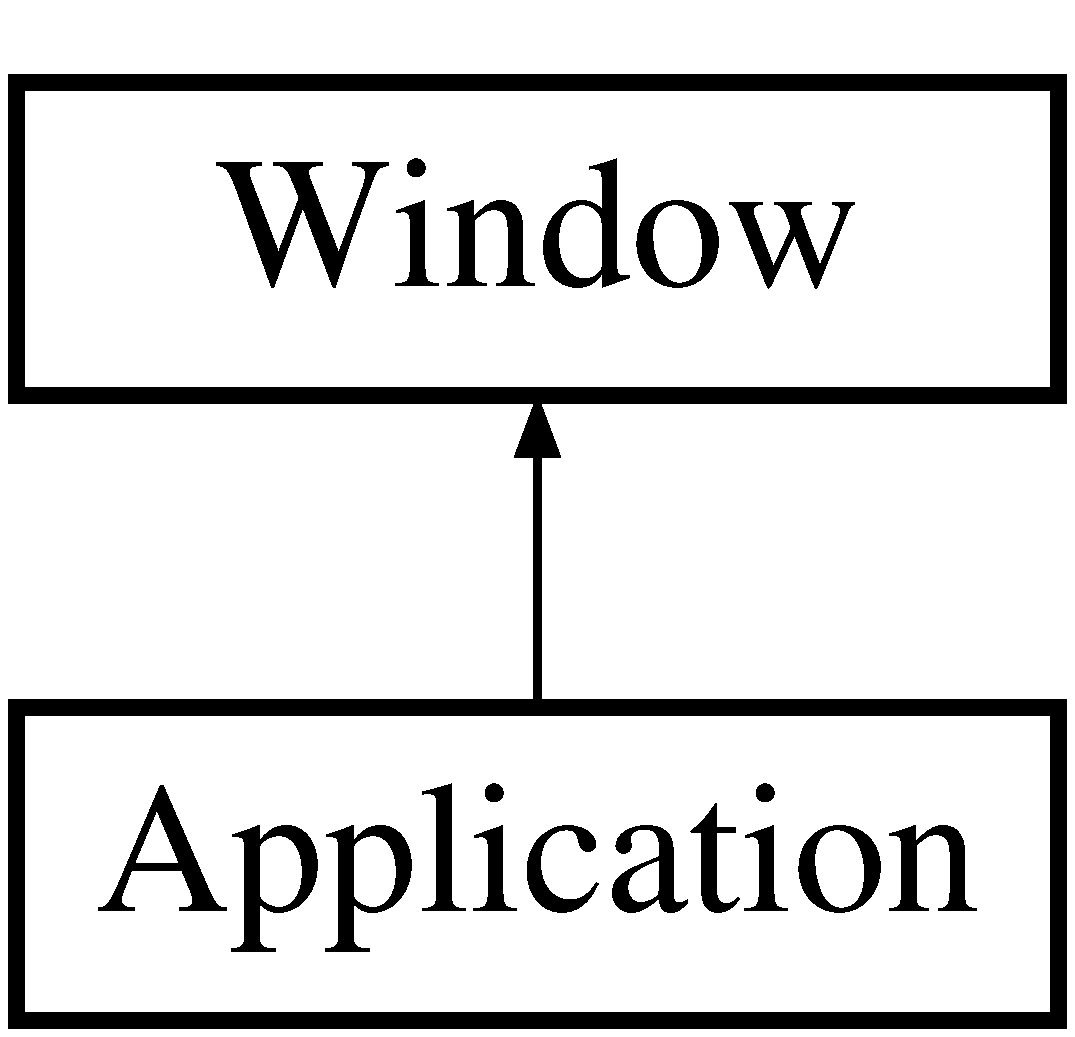
\includegraphics[height=2.000000cm]{classApplication}
\end{center}
\end{figure}
\subsection*{Public Member Functions}
\begin{DoxyCompactItemize}
\item 
\hypertarget{classApplication_a9ebed8021c5b7ebb5076371167d52b87}{{\bfseries Application} (\hyperlink{classProcessor}{Processor} $\ast$pro, \hyperlink{structOptions}{Options} opts)}\label{classApplication_a9ebed8021c5b7ebb5076371167d52b87}

\end{DoxyCompactItemize}
\subsection*{Protected Member Functions}
\begin{DoxyCompactItemize}
\item 
\hypertarget{classApplication_a29d82b42f3057ed83168b9b292608b97}{void {\bfseries drawing\-Loop} ()}\label{classApplication_a29d82b42f3057ed83168b9b292608b97}

\item 
\hypertarget{classApplication_a2a8493f4e82943b5958c8ac10c259746}{bool {\bfseries on\-\_\-delete\-\_\-event} (Gdk\-Event\-Any $\ast$event)}\label{classApplication_a2a8493f4e82943b5958c8ac10c259746}

\end{DoxyCompactItemize}


The documentation for this class was generated from the following files\-:\begin{DoxyCompactItemize}
\item 
headers/Application.\-hpp\item 
src/Application.\-cpp\end{DoxyCompactItemize}

\hypertarget{classArea}{\section{Area Class Reference}
\label{classArea}\index{Area@{Area}}
}
\subsection*{Public Member Functions}
\begin{DoxyCompactItemize}
\item 
\hypertarget{classArea_a001d8a1b7164d9ec28b5737c6a9a90c5}{{\bfseries Area} (cv\-::\-Rect R\-O\-I, cv\-::\-Mat bg, cv\-::\-Mat mask, int n\-Lines)}\label{classArea_a001d8a1b7164d9ec28b5737c6a9a90c5}

\item 
\hypertarget{classArea_a3470f64880b8647d16034b970e04c611}{cv\-::\-Mat \& {\bfseries get\-Territ} ()}\label{classArea_a3470f64880b8647d16034b970e04c611}

\item 
\hypertarget{classArea_a1f06bb9d7a4e372092df4b89a221a273}{cv\-::\-Rect \& {\bfseries get\-R\-O\-I} ()}\label{classArea_a1f06bb9d7a4e372092df4b89a221a273}

\item 
\hypertarget{classArea_aa726080825abc4673cc9ec9fc339983e}{int {\bfseries in\-Which\-Territ\-Is\-Point} (cv\-::\-Point2f p)}\label{classArea_aa726080825abc4673cc9ec9fc339983e}

\end{DoxyCompactItemize}
\subsection*{Protected Member Functions}
\begin{DoxyCompactItemize}
\item 
\hypertarget{classArea_a46be5cdc4414e28f3796b891dfb65278}{void {\bfseries one\-Line\-Territ} (cv\-::\-Mat bg)}\label{classArea_a46be5cdc4414e28f3796b891dfb65278}

\end{DoxyCompactItemize}


The documentation for this class was generated from the following files\-:\begin{DoxyCompactItemize}
\item 
headers/Area.\-hpp\item 
src/Area.\-cpp\end{DoxyCompactItemize}

\hypertarget{classAreaPreviewer}{\section{Area\-Previewer Class Reference}
\label{classAreaPreviewer}\index{Area\-Previewer@{Area\-Previewer}}
}
Inheritance diagram for Area\-Previewer\-:\begin{figure}[H]
\begin{center}
\leavevmode
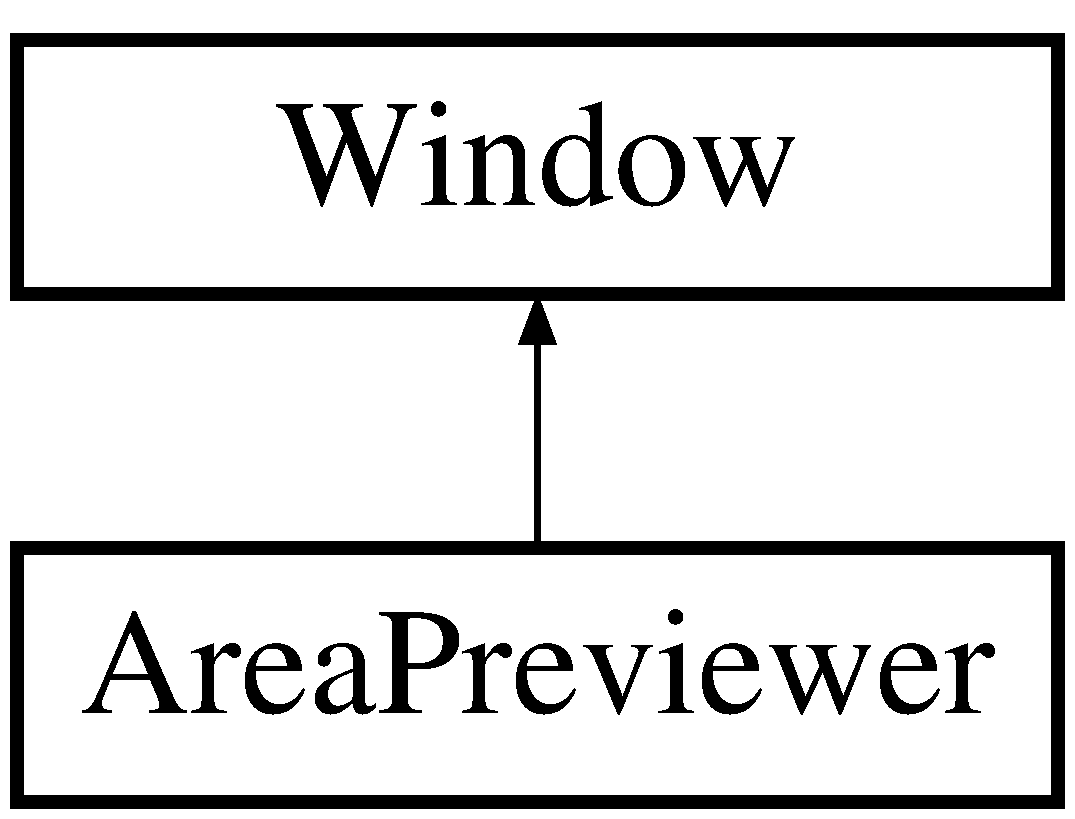
\includegraphics[height=2.000000cm]{classAreaPreviewer}
\end{center}
\end{figure}
\subsection*{Public Member Functions}
\begin{DoxyCompactItemize}
\item 
\hypertarget{classAreaPreviewer_a6b58de9ca1e93b329b593b050fa2e2c7}{void {\bfseries set\-Mat} (cv\-::\-Mat \&input)}\label{classAreaPreviewer_a6b58de9ca1e93b329b593b050fa2e2c7}

\end{DoxyCompactItemize}
\subsection*{Protected Member Functions}
\begin{DoxyCompactItemize}
\item 
\hypertarget{classAreaPreviewer_abb64dffa0d4806ec5c86ef89f1aedaa6}{bool {\bfseries on\-\_\-draw} ()}\label{classAreaPreviewer_abb64dffa0d4806ec5c86ef89f1aedaa6}

\item 
\hypertarget{classAreaPreviewer_aba5dd5876ce56a8fc6131b9fc37c47fc}{double {\bfseries scale\-Ratio} (int img\-W, int img\-H)}\label{classAreaPreviewer_aba5dd5876ce56a8fc6131b9fc37c47fc}

\item 
\hypertarget{classAreaPreviewer_a07370cec469cd7e09087f7ea9360864e}{bool {\bfseries on\-\_\-delete\-\_\-event} (Gdk\-Event\-Any $\ast$event)}\label{classAreaPreviewer_a07370cec469cd7e09087f7ea9360864e}

\end{DoxyCompactItemize}


The documentation for this class was generated from the following files\-:\begin{DoxyCompactItemize}
\item 
headers/Area\-Previewer.\-hpp\item 
src/Area\-Previewer.\-cpp\end{DoxyCompactItemize}

\hypertarget{classControlPanel}{\section{Control\-Panel Class Reference}
\label{classControlPanel}\index{Control\-Panel@{Control\-Panel}}
}
Inheritance diagram for Control\-Panel\-:\begin{figure}[H]
\begin{center}
\leavevmode
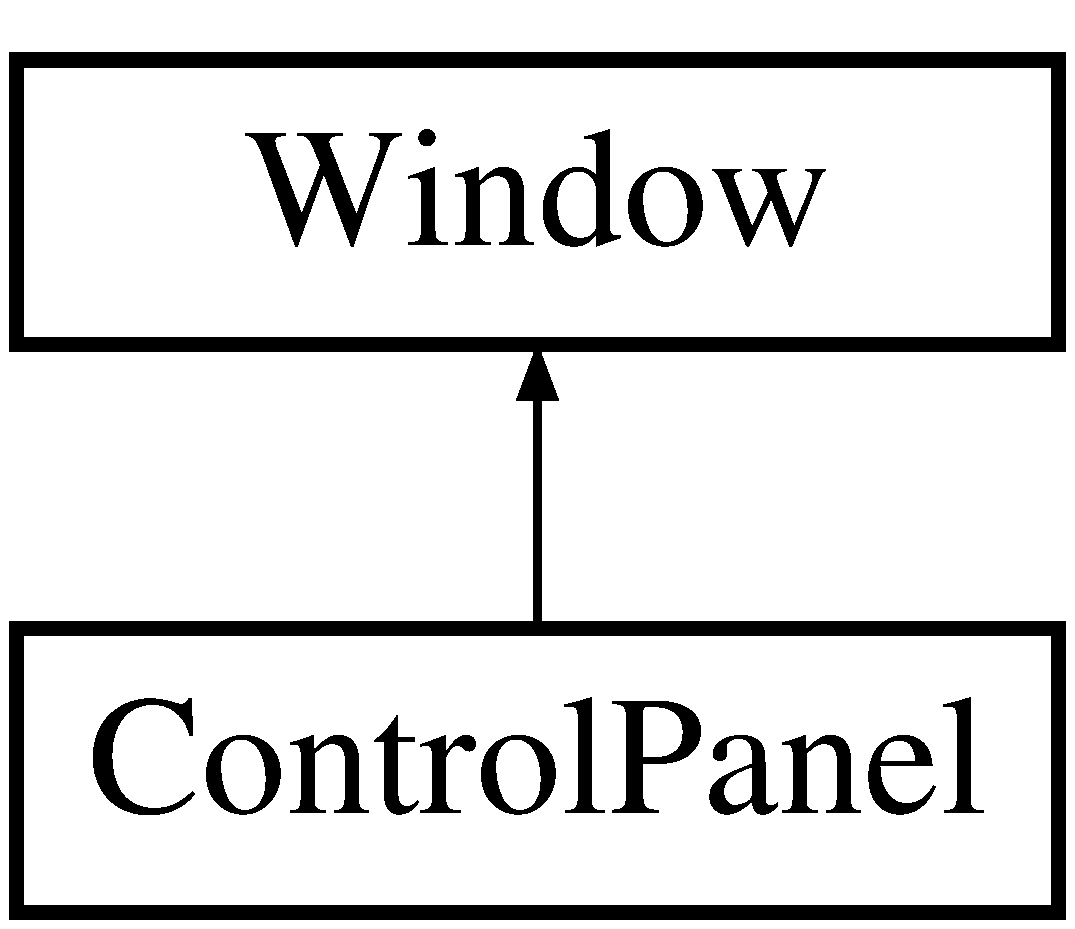
\includegraphics[height=2.000000cm]{classControlPanel}
\end{center}
\end{figure}
\subsection*{Public Member Functions}
\begin{DoxyCompactItemize}
\item 
\hypertarget{classControlPanel_a4d07f91393bf2d7a21f8d1124a778565}{{\bfseries Control\-Panel} (\hyperlink{classProcessor}{Processor} $\ast$pro, std\-::string $\ast$R\-O\-I, \hyperlink{structOptions}{Options} opts)}\label{classControlPanel_a4d07f91393bf2d7a21f8d1124a778565}

\item 
\hypertarget{classControlPanel_a7e05289f0fa706c91390507cbc620670}{void {\bfseries loop} ()}\label{classControlPanel_a7e05289f0fa706c91390507cbc620670}

\item 
\hypertarget{classControlPanel_a7cd10d20e519c32adb96c8a22d2c77cb}{void {\bfseries set\-Finished} (bool b)}\label{classControlPanel_a7cd10d20e519c32adb96c8a22d2c77cb}

\end{DoxyCompactItemize}
\subsection*{Protected Member Functions}
\begin{DoxyCompactItemize}
\item 
\hypertarget{classControlPanel_adee0e624d1b83a77e37b8e5dc21fe450}{bool {\bfseries on\-\_\-tick} ()}\label{classControlPanel_adee0e624d1b83a77e37b8e5dc21fe450}

\item 
\hypertarget{classControlPanel_a3a42b25d9cd44beca02b56858d2b3b64}{bool {\bfseries on\-\_\-update\-Progress} ()}\label{classControlPanel_a3a42b25d9cd44beca02b56858d2b3b64}

\item 
\hypertarget{classControlPanel_a51a884870108d1267d1ed631b3dea00e}{std\-::vector$<$ std\-::string $>$ {\bfseries sort\-Alpha} (std\-::vector$<$ std\-::string $>$ sort\-This)}\label{classControlPanel_a51a884870108d1267d1ed631b3dea00e}

\item 
\hypertarget{classControlPanel_af8e669ff68aac439a0de7f0687010a72}{void {\bfseries update\-Labels} ()}\label{classControlPanel_af8e669ff68aac439a0de7f0687010a72}

\item 
\hypertarget{classControlPanel_a648128d5b68bda3ab7768d7e63a6e763}{void {\bfseries on\-\_\-change\-Area} ()}\label{classControlPanel_a648128d5b68bda3ab7768d7e63a6e763}

\item 
\hypertarget{classControlPanel_af39aa7e898a29c9ed388b30dce9b6724}{void {\bfseries on\-\_\-finished} ()}\label{classControlPanel_af39aa7e898a29c9ed388b30dce9b6724}

\end{DoxyCompactItemize}


The documentation for this class was generated from the following files\-:\begin{DoxyCompactItemize}
\item 
headers/Control\-Panel.\-hpp\item 
src/Control\-Panel.\-cpp\end{DoxyCompactItemize}

\hypertarget{classDecorator}{\section{Decorator Class Reference}
\label{classDecorator}\index{Decorator@{Decorator}}
}
\subsection*{Public Member Functions}
\begin{DoxyCompactItemize}
\item 
\hypertarget{classDecorator_a2c55e2aed9fe25a5be7fe5f2a8705d66}{{\bfseries Decorator} (std\-::vector$<$ \hyperlink{classTracker}{Tracker} $>$ $\ast$trackers, cv\-::\-Size img\-Size)}\label{classDecorator_a2c55e2aed9fe25a5be7fe5f2a8705d66}

\item 
\hypertarget{classDecorator_a4da99b258d95fe21772d534e915a4765}{void {\bfseries get\-Decorated\-Frame} (cv\-::\-Mat \&frame)}\label{classDecorator_a4da99b258d95fe21772d534e915a4765}

\item 
\hypertarget{classDecorator_a162529f4b2bd01f0023910b839f80b6e}{void {\bfseries new\-Frame} (cv\-::\-Mat \&frame)}\label{classDecorator_a162529f4b2bd01f0023910b839f80b6e}

\item 
\hypertarget{classDecorator_a2184982851eaca7055c9bf46d5c5a7c5}{void {\bfseries plot} (int i)}\label{classDecorator_a2184982851eaca7055c9bf46d5c5a7c5}

\end{DoxyCompactItemize}
\subsection*{Protected Member Functions}
\begin{DoxyCompactItemize}
\item 
\hypertarget{classDecorator_a5219da97e4c259f8fa36d55b11d245de}{void {\bfseries make\-Static\-Overlay} ()}\label{classDecorator_a5219da97e4c259f8fa36d55b11d245de}

\end{DoxyCompactItemize}


The documentation for this class was generated from the following files\-:\begin{DoxyCompactItemize}
\item 
headers/Decorator.\-hpp\item 
src/Decorator.\-cpp\end{DoxyCompactItemize}

\hypertarget{classDrawingArea}{\section{Drawing\-Area Class Reference}
\label{classDrawingArea}\index{Drawing\-Area@{Drawing\-Area}}
}
Inheritance diagram for Drawing\-Area\-:\begin{figure}[H]
\begin{center}
\leavevmode
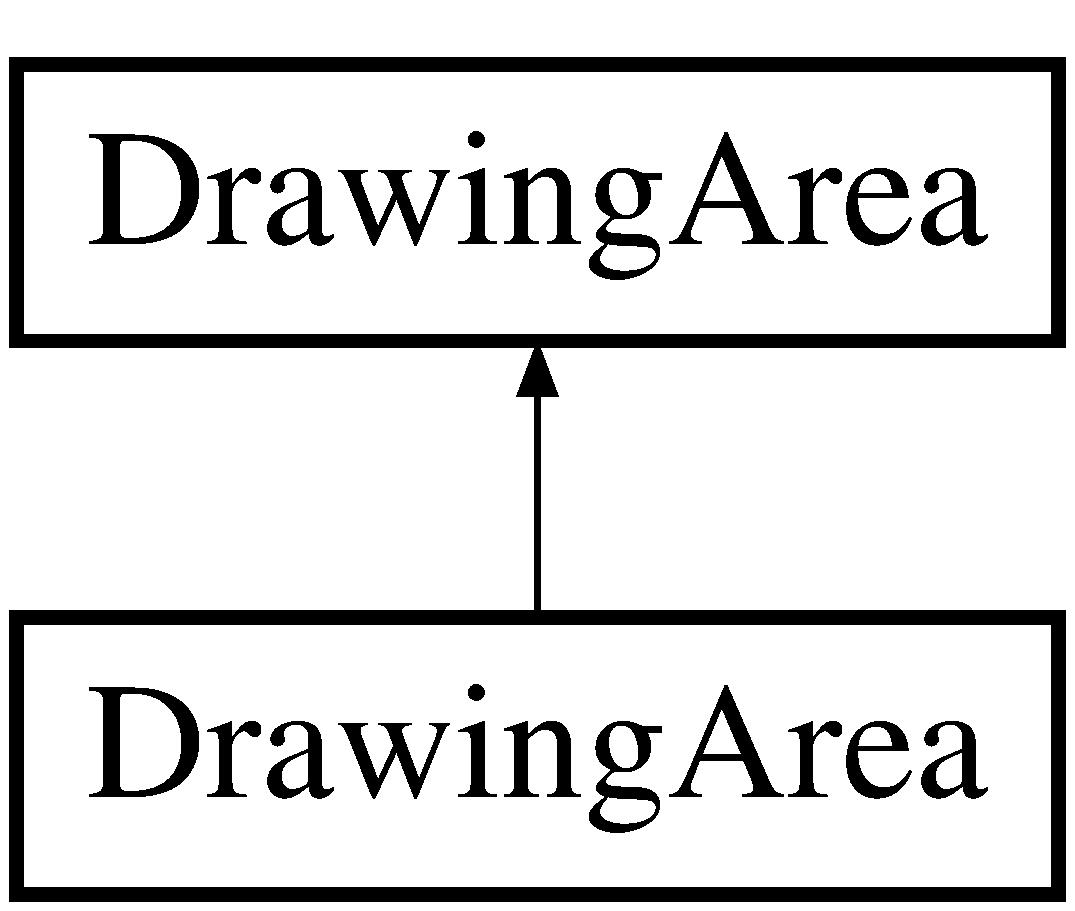
\includegraphics[height=2.000000cm]{classDrawingArea}
\end{center}
\end{figure}
\subsection*{Public Member Functions}
\begin{DoxyCompactItemize}
\item 
\hypertarget{classDrawingArea_a4b84cb4d43b4cd64ffa3055525d1d52e}{{\bfseries Drawing\-Area} (\hyperlink{classProcessor}{Processor} $\ast$pro, std\-::string $\ast$R\-O\-I)}\label{classDrawingArea_a4b84cb4d43b4cd64ffa3055525d1d52e}

\item 
\hypertarget{classDrawingArea_a9a2d199506c09591e756045c55151eef}{void {\bfseries loop} ()}\label{classDrawingArea_a9a2d199506c09591e756045c55151eef}

\end{DoxyCompactItemize}
\subsection*{Protected Member Functions}
\begin{DoxyCompactItemize}
\item 
\hypertarget{classDrawingArea_a23196e37bb7fd9780601cc2c22abdae1}{double {\bfseries scale\-Ratio} (int img\-W, int img\-H)}\label{classDrawingArea_a23196e37bb7fd9780601cc2c22abdae1}

\item 
\hypertarget{classDrawingArea_a4b228965df0cdfe4df0bfe2d63ea868a}{void {\bfseries render} ()}\label{classDrawingArea_a4b228965df0cdfe4df0bfe2d63ea868a}

\item 
\hypertarget{classDrawingArea_a38dc7e682edc21fff94c79760d500122}{void {\bfseries make\-New\-Pixbuf} ()}\label{classDrawingArea_a38dc7e682edc21fff94c79760d500122}

\item 
\hypertarget{classDrawingArea_aed51b64e5b9c5a63f2a3b448eadbf611}{bool {\bfseries test} ()}\label{classDrawingArea_aed51b64e5b9c5a63f2a3b448eadbf611}

\end{DoxyCompactItemize}


The documentation for this class was generated from the following files\-:\begin{DoxyCompactItemize}
\item 
headers/Drawing\-Area.\-hpp\item 
src/Drawing\-Area.\-cpp\end{DoxyCompactItemize}

\hypertarget{classFeatureClassifier}{\section{Feature\-Classifier Class Reference}
\label{classFeatureClassifier}\index{Feature\-Classifier@{Feature\-Classifier}}
}
\subsection*{Public Member Functions}
\begin{DoxyCompactItemize}
\item 
\hypertarget{classFeatureClassifier_adc9bc89baf4d4abe675c6b1955d188c0}{{\bfseries Feature\-Classifier} (int round\-To\-Train)}\label{classFeatureClassifier_adc9bc89baf4d4abe675c6b1955d188c0}

\item 
\hypertarget{classFeatureClassifier_a3667ca84e2ab7e05becb01dc1b2e4e17}{void {\bfseries run} (std\-::vector$<$ std\-::vector$<$ cv\-::\-Point $>$ $>$ \&contours, cv\-::\-Mat \&img)}\label{classFeatureClassifier_a3667ca84e2ab7e05becb01dc1b2e4e17}

\item 
\hypertarget{classFeatureClassifier_ad01ef2cbf47cb4ad255c26a4ddbbd1f4}{bool {\bfseries is\-Trained} ()}\label{classFeatureClassifier_ad01ef2cbf47cb4ad255c26a4ddbbd1f4}

\item 
\hypertarget{classFeatureClassifier_a4c21690cf961f1023b6d1601c8b32a23}{float {\bfseries trained\-Fract} ()}\label{classFeatureClassifier_a4c21690cf961f1023b6d1601c8b32a23}

\item 
\hypertarget{classFeatureClassifier_aba2276bc6553b11f08139f8d0586c763}{float {\bfseries get\-L} ()}\label{classFeatureClassifier_aba2276bc6553b11f08139f8d0586c763}

\item 
\hypertarget{classFeatureClassifier_a3f52d77c51b43935faddfcd1db02dcc6}{cv\-::\-Point2f {\bfseries get\-Position} ()}\label{classFeatureClassifier_a3f52d77c51b43935faddfcd1db02dcc6}

\end{DoxyCompactItemize}
\subsection*{Protected Member Functions}
\begin{DoxyCompactItemize}
\item 
\hypertarget{classFeatureClassifier_a2ca27db91b6f241c680f37409402bc58}{void {\bfseries make\-Mini\-Img} (std\-::vector$<$ cv\-::\-Point $>$ \&contour, cv\-::\-Mat \&mini\-I\-M\-G, cv\-::\-Mat \&img)}\label{classFeatureClassifier_a2ca27db91b6f241c680f37409402bc58}

\item 
\hypertarget{classFeatureClassifier_ae742d63d70d0621b5c7fba21336d0b6b}{void {\bfseries make\-Features} (std\-::vector$<$ double $>$ \&, std\-::vector$<$ cv\-::\-Point $>$ \&contour, cv\-::\-Mat \&mini\-I\-M\-G)}\label{classFeatureClassifier_ae742d63d70d0621b5c7fba21336d0b6b}

\item 
\hypertarget{classFeatureClassifier_abdb6cbcaa98db6bfad9d520712790172}{cv\-::\-Point2f {\bfseries update\-Position} (cv\-::\-Point2f center)}\label{classFeatureClassifier_abdb6cbcaa98db6bfad9d520712790172}

\item 
\hypertarget{classFeatureClassifier_afb99e30afeb76f0fc015f77ceaea6b83}{float {\bfseries calc\-Likelyhood} (std\-::vector$<$ double $>$ \&vect)}\label{classFeatureClassifier_afb99e30afeb76f0fc015f77ceaea6b83}

\item 
\hypertarget{classFeatureClassifier_afabb0d18b79b81103ec01fe8f653b2b3}{void {\bfseries update\-Mean\-S\-D} (std\-::vector$<$ double $>$ \&vect)}\label{classFeatureClassifier_afabb0d18b79b81103ec01fe8f653b2b3}

\end{DoxyCompactItemize}


The documentation for this class was generated from the following files\-:\begin{DoxyCompactItemize}
\item 
headers/Feature\-Classifier.\-hpp\item 
src/Feature\-Classifier.\-cpp\end{DoxyCompactItemize}

\hypertarget{classForegroundExtractor}{\section{Foreground\-Extractor Class Reference}
\label{classForegroundExtractor}\index{Foreground\-Extractor@{Foreground\-Extractor}}
}
\subsection*{Public Member Functions}
\begin{DoxyCompactItemize}
\item 
\hypertarget{classForegroundExtractor_a8ce9cd0c7aed353cc9e52175c1179256}{{\bfseries Foreground\-Extractor} (int round\-To\-Train)}\label{classForegroundExtractor_a8ce9cd0c7aed353cc9e52175c1179256}

\item 
\hypertarget{classForegroundExtractor_ad6e362a0ee050f99dc565d3a1683f9db}{int {\bfseries run} (cv\-::\-Mat \&img, cv\-::\-Mat \&mot, double motion\-Q, bool was\-Ambig, std\-::vector$<$ std\-::vector$<$ cv\-::\-Point $>$ $>$ \&valid\-Contours)}\label{classForegroundExtractor_ad6e362a0ee050f99dc565d3a1683f9db}

\item 
\hypertarget{classForegroundExtractor_ad70860dab3af9c6519974da0e1974c44}{bool {\bfseries is\-Trained} ()}\label{classForegroundExtractor_ad70860dab3af9c6519974da0e1974c44}

\item 
\hypertarget{classForegroundExtractor_a8f75097646a2804a07726aa1cb5b2596}{float {\bfseries trained\-Fract} ()}\label{classForegroundExtractor_a8f75097646a2804a07726aa1cb5b2596}

\end{DoxyCompactItemize}
\subsection*{Protected Member Functions}
\begin{DoxyCompactItemize}
\item 
\hypertarget{classForegroundExtractor_a176a1ac5cb57e525d59b761b68d1d4e4}{void {\bfseries update\-Training\-Rate} ()}\label{classForegroundExtractor_a176a1ac5cb57e525d59b761b68d1d4e4}

\item 
\hypertarget{classForegroundExtractor_a4ed8865b9e063b29f7e687e37193588d}{void {\bfseries merge\-Contours} (cv\-::\-Mat \&img, std\-::vector$<$ std\-::vector$<$ cv\-::\-Point $>$ $>$ \&contours)}\label{classForegroundExtractor_a4ed8865b9e063b29f7e687e37193588d}

\item 
\hypertarget{classForegroundExtractor_a1e6a870b80ad619cd8fb77cd1c3441da}{void {\bfseries remove\-Large\-Contours} (std\-::vector$<$ std\-::vector$<$ cv\-::\-Point $>$ $>$ \&contours, double max)}\label{classForegroundExtractor_a1e6a870b80ad619cd8fb77cd1c3441da}

\end{DoxyCompactItemize}


The documentation for this class was generated from the following files\-:\begin{DoxyCompactItemize}
\item 
headers/Foreground\-Extractor.\-hpp\item 
src/Foreground\-Extractor.\-cpp\end{DoxyCompactItemize}

\hypertarget{classMotionSensor}{\section{Motion\-Sensor Class Reference}
\label{classMotionSensor}\index{Motion\-Sensor@{Motion\-Sensor}}
}
\subsection*{Public Member Functions}
\begin{DoxyCompactItemize}
\item 
\hypertarget{classMotionSensor_af2f1013fcff9a706249bfa0043e1cca1}{{\bfseries Motion\-Sensor} (int sensitivity, cv\-::\-Mat \&mask)}\label{classMotionSensor_af2f1013fcff9a706249bfa0043e1cca1}

\item 
\hypertarget{classMotionSensor_a6dc19202befbb6eac2fb7a4d1d3d96e5}{double {\bfseries run} (cv\-::\-Mat \&img, cv\-::\-Mat \&out)}\label{classMotionSensor_a6dc19202befbb6eac2fb7a4d1d3d96e5}

\end{DoxyCompactItemize}


The documentation for this class was generated from the following files\-:\begin{DoxyCompactItemize}
\item 
headers/Motion\-Sensor.\-hpp\item 
src/Motion\-Sensor.\-cpp\end{DoxyCompactItemize}

\hypertarget{classOptionParser}{\section{Option\-Parser Class Reference}
\label{classOptionParser}\index{Option\-Parser@{Option\-Parser}}
}
\subsection*{Public Member Functions}
\begin{DoxyCompactItemize}
\item 
\hypertarget{classOptionParser_ad4e77fb879939e1be9b0d3db9e3d9c1d}{{\bfseries Option\-Parser} (int argc, char $\ast$$\ast$argv)}\label{classOptionParser_ad4e77fb879939e1be9b0d3db9e3d9c1d}

\item 
\hypertarget{classOptionParser_aaf8c1744ffbeabf4d6cd8cf2b7aced3c}{\hyperlink{structOptions}{Options} {\bfseries Get\-Options} ()}\label{classOptionParser_aaf8c1744ffbeabf4d6cd8cf2b7aced3c}

\item 
\hypertarget{classOptionParser_a97c8596b8d61a343946646d0cda304d3}{bool {\bfseries check\-Options} ()}\label{classOptionParser_a97c8596b8d61a343946646d0cda304d3}

\end{DoxyCompactItemize}
\subsection*{Protected Member Functions}
\begin{DoxyCompactItemize}
\item 
\hypertarget{classOptionParser_a0aa28808c4158c44b280023a5b310448}{void {\bfseries help} ()}\label{classOptionParser_a0aa28808c4158c44b280023a5b310448}

\end{DoxyCompactItemize}


The documentation for this class was generated from the following files\-:\begin{DoxyCompactItemize}
\item 
headers/Option\-Parser.\-hpp\item 
src/Option\-Parser.\-cpp\end{DoxyCompactItemize}

\hypertarget{structOptions}{\section{Options Struct Reference}
\label{structOptions}\index{Options@{Options}}
}
\subsection*{Public Attributes}
\begin{DoxyCompactItemize}
\item 
\hypertarget{structOptions_a815c1f3e2dcdece0ef1ee4f27234a758}{std\-::string {\bfseries video\-File}}\label{structOptions_a815c1f3e2dcdece0ef1ee4f27234a758}

\item 
\hypertarget{structOptions_a428a0a33d32984f5b7425b2d11ed3f92}{std\-::string {\bfseries out\-Dir}}\label{structOptions_a428a0a33d32984f5b7425b2d11ed3f92}

\item 
\hypertarget{structOptions_a28bb07e52ddc7413c7b0710a9b3c2b17}{int {\bfseries web\-Cam\-Idx}}\label{structOptions_a28bb07e52ddc7413c7b0710a9b3c2b17}

\item 
\hypertarget{structOptions_a9d688783bef0f0854dc9168fa5471adc}{unsigned int {\bfseries n\-Dishes}}\label{structOptions_a9d688783bef0f0854dc9168fa5471adc}

\item 
\hypertarget{structOptions_aa63b1b70e4954acf9af48225c9975c11}{int {\bfseries n\-Line\-Per\-Dishes}}\label{structOptions_aa63b1b70e4954acf9af48225c9975c11}

\item 
\hypertarget{structOptions_a4256287c28547e3c8f44e853de41fbfc}{int {\bfseries motion\-Sensitivity}}\label{structOptions_a4256287c28547e3c8f44e853de41fbfc}

\item 
\hypertarget{structOptions_acd0bf1ebddabc64d6824209d428de1ee}{int {\bfseries M\-O\-G\-Training\-Rounds}}\label{structOptions_acd0bf1ebddabc64d6824209d428de1ee}

\item 
\hypertarget{structOptions_ad2c3435e77c0a66e10c3f541dfb66b0c}{bool {\bfseries result\-File}}\label{structOptions_ad2c3435e77c0a66e10c3f541dfb66b0c}

\item 
\hypertarget{structOptions_a21fd208622a325f0bfaa6eca9a3c1de9}{bool {\bfseries videos\-Output}}\label{structOptions_a21fd208622a325f0bfaa6eca9a3c1de9}

\item 
\hypertarget{structOptions_a799fecf713718ceb2399195742cc6b5b}{bool {\bfseries all\-Frame\-Output}}\label{structOptions_a799fecf713718ceb2399195742cc6b5b}

\item 
\hypertarget{structOptions_a51e700e7824100576ebb4655145afc08}{bool {\bfseries write\-First\-Picture}}\label{structOptions_a51e700e7824100576ebb4655145afc08}

\item 
\hypertarget{structOptions_a808d607657e61484aa1eb3f57ad0f6c7}{bool {\bfseries has\-G\-U\-I}}\label{structOptions_a808d607657e61484aa1eb3f57ad0f6c7}

\item 
\hypertarget{structOptions_aada243e50c7ec08cf7cf578685bbe074}{bool {\bfseries has\-Assistant}}\label{structOptions_aada243e50c7ec08cf7cf578685bbe074}

\end{DoxyCompactItemize}


The documentation for this struct was generated from the following file\-:\begin{DoxyCompactItemize}
\item 
headers/option\-Structure.\-hpp\end{DoxyCompactItemize}

\hypertarget{classPageAreaMaker}{\section{Page\-Area\-Maker Class Reference}
\label{classPageAreaMaker}\index{Page\-Area\-Maker@{Page\-Area\-Maker}}
}
Inheritance diagram for Page\-Area\-Maker\-:\begin{figure}[H]
\begin{center}
\leavevmode
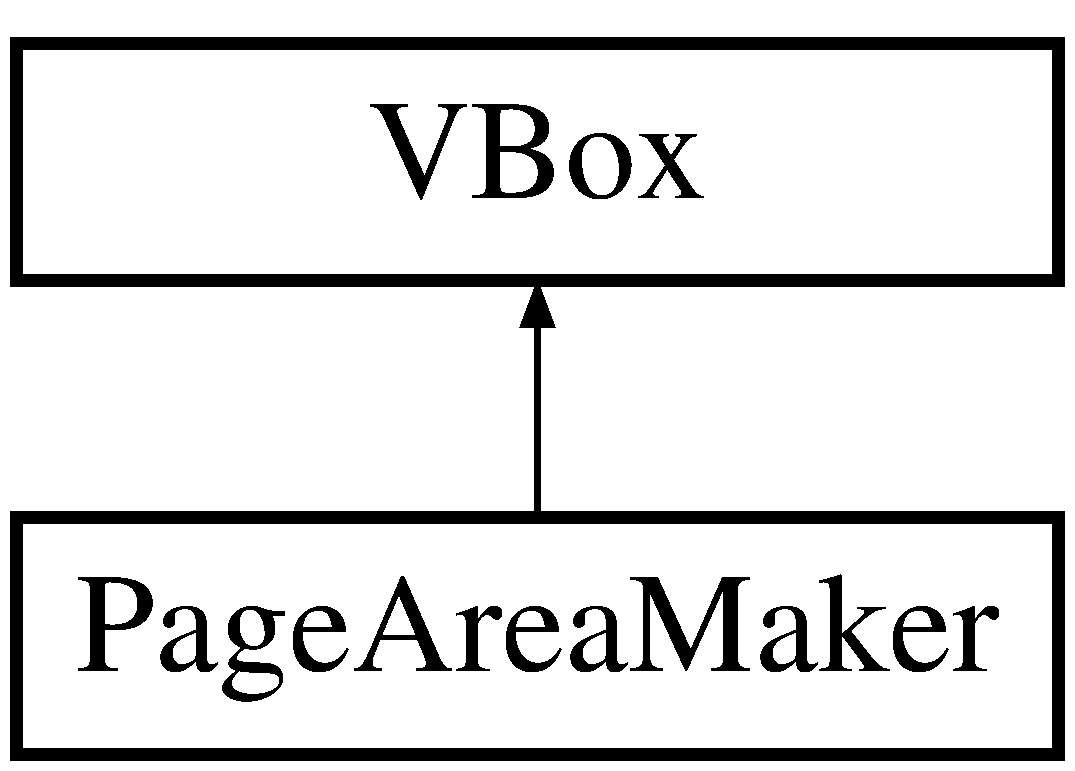
\includegraphics[height=2.000000cm]{classPageAreaMaker}
\end{center}
\end{figure}
\subsection*{Public Member Functions}
\begin{DoxyCompactItemize}
\item 
\hypertarget{classPageAreaMaker_a34cc8b3883e08accf0a0f7545ed2db1f}{{\bfseries Page\-Area\-Maker} (Gtk\-::\-Assistant $\ast$parent, \hyperlink{structOptions}{Options} $\ast$opts, \hyperlink{classVideoGrabber}{Video\-Grabber} $\ast$video\-Grab)}\label{classPageAreaMaker_a34cc8b3883e08accf0a0f7545ed2db1f}

\item 
\hypertarget{classPageAreaMaker_abace3043eafde9e50c13a26e8b27b2d6}{Glib\-::ustring {\bfseries get\-\_\-title} ()}\label{classPageAreaMaker_abace3043eafde9e50c13a26e8b27b2d6}

\item 
\hypertarget{classPageAreaMaker_a72aa63471d73a79e4ce94c939b06cc99}{void {\bfseries hide\-Mode\-Boxes} ()}\label{classPageAreaMaker_a72aa63471d73a79e4ce94c939b06cc99}

\end{DoxyCompactItemize}
\subsection*{Protected Member Functions}
\begin{DoxyCompactItemize}
\item 
\hypertarget{classPageAreaMaker_af30ee07c1b3627c94f0a429b6723773a}{void {\bfseries on\-\_\-mode\-\_\-changed} ()}\label{classPageAreaMaker_af30ee07c1b3627c94f0a429b6723773a}

\item 
\hypertarget{classPageAreaMaker_a8a5e4e1bd2f7cd889d5d475a04d7bb63}{void {\bfseries update\-Opts} ()}\label{classPageAreaMaker_a8a5e4e1bd2f7cd889d5d475a04d7bb63}

\item 
\hypertarget{classPageAreaMaker_a63eba0d0aff4ad489cfc6d9231614c1a}{void {\bfseries make\-Preview} ()}\label{classPageAreaMaker_a63eba0d0aff4ad489cfc6d9231614c1a}

\end{DoxyCompactItemize}


The documentation for this class was generated from the following files\-:\begin{DoxyCompactItemize}
\item 
headers/Page\-Area\-Maker.\-hpp\item 
src/Page\-Area\-Maker.\-cpp\end{DoxyCompactItemize}

\hypertarget{classPageOutput}{\section{Page\-Output Class Reference}
\label{classPageOutput}\index{Page\-Output@{Page\-Output}}
}
Inheritance diagram for Page\-Output\-:\begin{figure}[H]
\begin{center}
\leavevmode
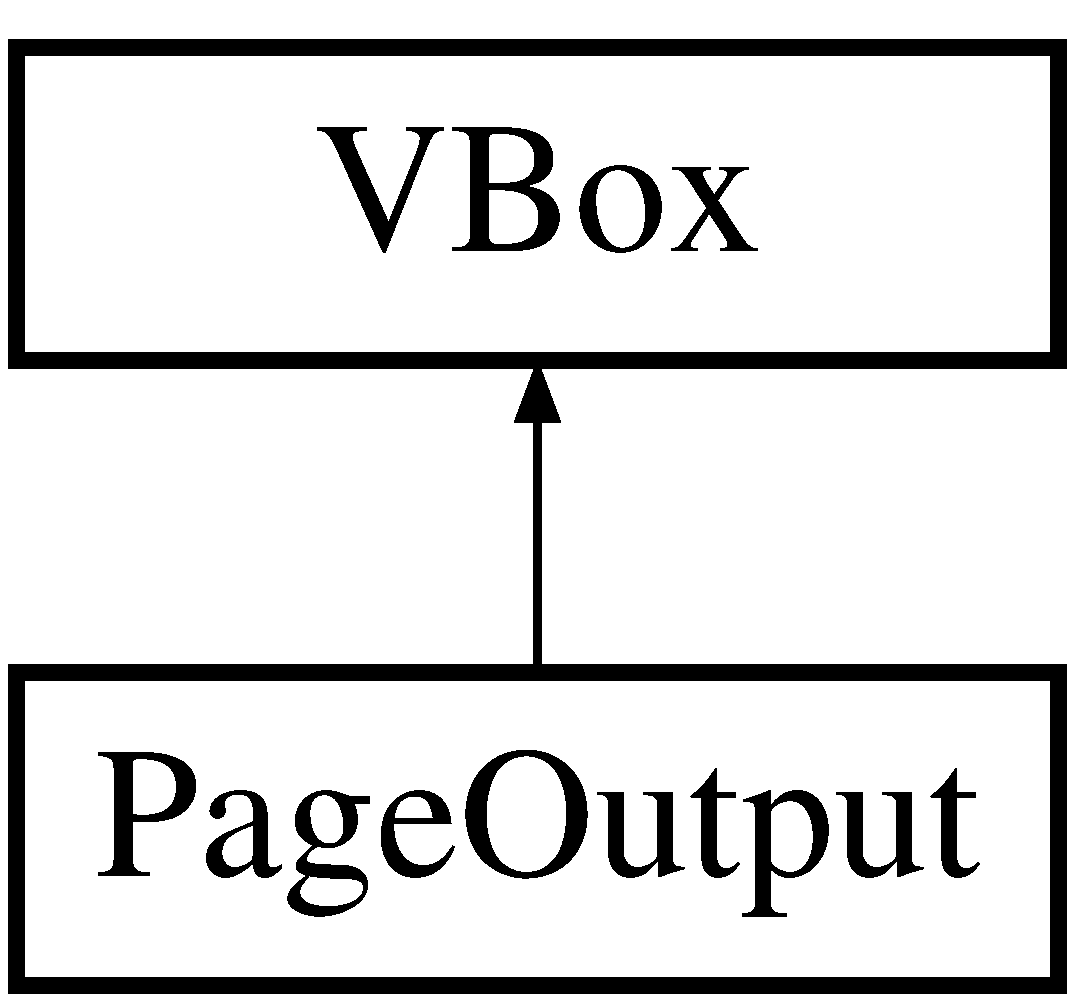
\includegraphics[height=2.000000cm]{classPageOutput}
\end{center}
\end{figure}
\subsection*{Public Member Functions}
\begin{DoxyCompactItemize}
\item 
\hypertarget{classPageOutput_acbea1db510bfecfba8afdd91e1b802cc}{{\bfseries Page\-Output} (Gtk\-::\-Assistant $\ast$parent, \hyperlink{structOptions}{Options} $\ast$opts, \hyperlink{classVideoGrabber}{Video\-Grabber} $\ast$video\-Grab)}\label{classPageOutput_acbea1db510bfecfba8afdd91e1b802cc}

\item 
\hypertarget{classPageOutput_a3d1a65461ace501e4a3767ff3794b283}{Glib\-::ustring {\bfseries get\-\_\-title} ()}\label{classPageOutput_a3d1a65461ace501e4a3767ff3794b283}

\end{DoxyCompactItemize}
\subsection*{Protected Member Functions}
\begin{DoxyCompactItemize}
\item 
\hypertarget{classPageOutput_a91541fd8cb13443f97989f1989ffc3b8}{void {\bfseries on\-\_\-pick\-Folder} ()}\label{classPageOutput_a91541fd8cb13443f97989f1989ffc3b8}

\item 
\hypertarget{classPageOutput_ad37e7bfcc6ed09a50c601eb89219897a}{void {\bfseries on\-\_\-update} ()}\label{classPageOutput_ad37e7bfcc6ed09a50c601eb89219897a}

\item 
\hypertarget{classPageOutput_a10a3304731ccf58f892a5c336a119d1a}{void {\bfseries on\-\_\-start} ()}\label{classPageOutput_a10a3304731ccf58f892a5c336a119d1a}

\end{DoxyCompactItemize}


The documentation for this class was generated from the following files\-:\begin{DoxyCompactItemize}
\item 
headers/Page\-Output.\-hpp\item 
src/Page\-Output.\-cpp\end{DoxyCompactItemize}

\hypertarget{classPageProcessPars}{\section{Page\-Process\-Pars Class Reference}
\label{classPageProcessPars}\index{Page\-Process\-Pars@{Page\-Process\-Pars}}
}
Inheritance diagram for Page\-Process\-Pars\-:\begin{figure}[H]
\begin{center}
\leavevmode
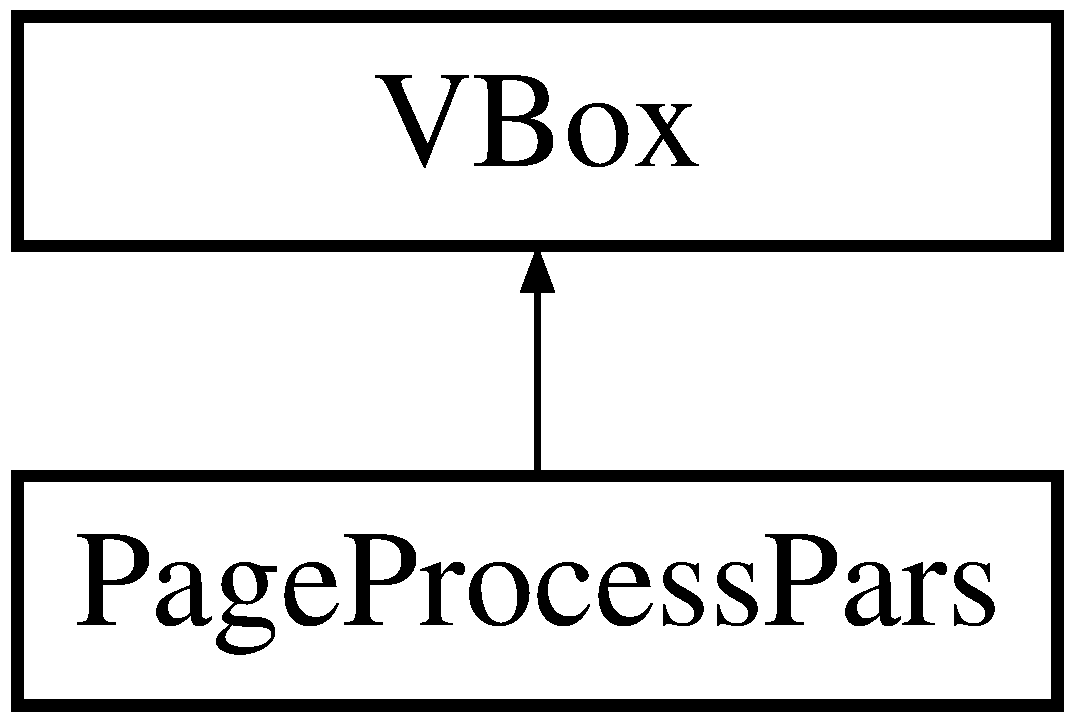
\includegraphics[height=2.000000cm]{classPageProcessPars}
\end{center}
\end{figure}
\subsection*{Public Member Functions}
\begin{DoxyCompactItemize}
\item 
\hypertarget{classPageProcessPars_aaa45dcfab0e838bab662e66df55e6019}{{\bfseries Page\-Process\-Pars} (Gtk\-::\-Assistant $\ast$parent, \hyperlink{structOptions}{Options} $\ast$opts, \hyperlink{classVideoGrabber}{Video\-Grabber} $\ast$video\-Grab)}\label{classPageProcessPars_aaa45dcfab0e838bab662e66df55e6019}

\item 
\hypertarget{classPageProcessPars_a2c272c5932c1a573b6e9824e44d50f90}{Glib\-::ustring {\bfseries get\-\_\-title} ()}\label{classPageProcessPars_a2c272c5932c1a573b6e9824e44d50f90}

\end{DoxyCompactItemize}
\subsection*{Protected Member Functions}
\begin{DoxyCompactItemize}
\item 
\hypertarget{classPageProcessPars_af8e1ac883944e4807932ed8f734bcbfe}{void {\bfseries update\-Opts} ()}\label{classPageProcessPars_af8e1ac883944e4807932ed8f734bcbfe}

\end{DoxyCompactItemize}


The documentation for this class was generated from the following files\-:\begin{DoxyCompactItemize}
\item 
headers/Page\-Process\-Pars.\-hpp\item 
src/Page\-Process\-Pars.\-cpp\end{DoxyCompactItemize}

\hypertarget{classPageVideoInput}{\section{Page\-Video\-Input Class Reference}
\label{classPageVideoInput}\index{Page\-Video\-Input@{Page\-Video\-Input}}
}
Inheritance diagram for Page\-Video\-Input\-:\begin{figure}[H]
\begin{center}
\leavevmode
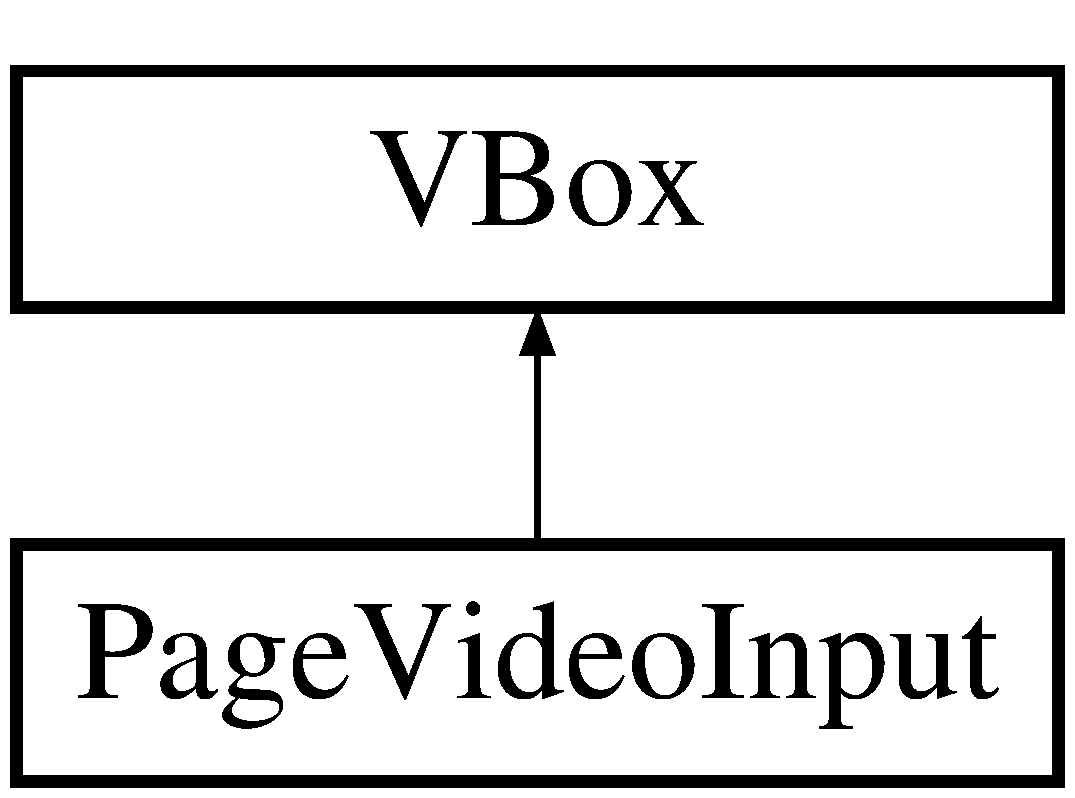
\includegraphics[height=2.000000cm]{classPageVideoInput}
\end{center}
\end{figure}
\subsection*{Public Member Functions}
\begin{DoxyCompactItemize}
\item 
\hypertarget{classPageVideoInput_a2f04dc94991b0eef4bce981593c2b63a}{{\bfseries Page\-Video\-Input} (Gtk\-::\-Assistant $\ast$parent, \hyperlink{structOptions}{Options} $\ast$opts, \hyperlink{classVideoGrabber}{Video\-Grabber} $\ast$video\-Grab)}\label{classPageVideoInput_a2f04dc94991b0eef4bce981593c2b63a}

\item 
\hypertarget{classPageVideoInput_aa882055b9fec8bdf207755ffba032f2d}{Glib\-::ustring {\bfseries get\-\_\-title} ()}\label{classPageVideoInput_aa882055b9fec8bdf207755ffba032f2d}

\end{DoxyCompactItemize}
\subsection*{Protected Member Functions}
\begin{DoxyCompactItemize}
\item 
\hypertarget{classPageVideoInput_a2687b087ef936f3b286092a2d3dc8abb}{void {\bfseries on\-\_\-load\-File\-\_\-clicked} ()}\label{classPageVideoInput_a2687b087ef936f3b286092a2d3dc8abb}

\end{DoxyCompactItemize}


The documentation for this class was generated from the following files\-:\begin{DoxyCompactItemize}
\item 
headers/Page\-Video\-Input.\-hpp\item 
src/Page\-Video\-Input.\-cpp\end{DoxyCompactItemize}

\hypertarget{classProcessor}{\section{Processor Class Reference}
\label{classProcessor}\index{Processor@{Processor}}
}


{\ttfamily \#include $<$Processor.\-hpp$>$}

\subsection*{Public Member Functions}
\begin{DoxyCompactItemize}
\item 
\hyperlink{classProcessor_acaeabaa5d52c03c6a112118c49196dbf}{Processor} (\hyperlink{structOptions}{Options} options, \hyperlink{classVideoGrabber}{Video\-Grabber} video\-Grab, bool has\-G\-U\-I=false, cv\-::\-Mat $\ast$preview=N\-U\-L\-L)
\item 
virtual \hyperlink{classProcessor_acf37952c5b420d4e903a512571678692}{$\sim$\-Processor} ()
\item 
void \hyperlink{classProcessor_a68a22b324edc0ef64f9b3cd513b1e778}{track} ()
\item 
\hypertarget{classProcessor_a094fa536ef16ea3662c3377928115275}{void {\bfseries set\-R\-O\-I\-For\-G\-U\-I} (std\-::string R\-O\-I\-Name)}\label{classProcessor_a094fa536ef16ea3662c3377928115275}

\item 
\hypertarget{classProcessor_a387474f67ba72edc1ed8aaed34f1d112}{bool {\bfseries get\-Deco} (cv\-::\-Mat \&out)}\label{classProcessor_a387474f67ba72edc1ed8aaed34f1d112}

\item 
\hypertarget{classProcessor_afeff66ffd64ccf90acf26a39650a1c72}{float $\ast$ {\bfseries get\-Tracker\-X\-Y\-Trained\-Territ} ()}\label{classProcessor_afeff66ffd64ccf90acf26a39650a1c72}

\item 
\hypertarget{classProcessor_af36c27815deeae7607e37e14fe5e2a02}{int $\ast$ {\bfseries get\-Tracker\-W\-H\-X\-Y\-\_\-\-R\-O\-I} ()}\label{classProcessor_af36c27815deeae7607e37e14fe5e2a02}

\item 
\hypertarget{classProcessor_af2dc8564c9f51b94c354ca27ef4ef0f6}{void {\bfseries set\-Is\-Finished} (bool b)}\label{classProcessor_af2dc8564c9f51b94c354ca27ef4ef0f6}

\item 
\hypertarget{classProcessor_a7e82f65e87756a77c1730aa3f0f808bb}{bool {\bfseries get\-Is\-Finished} ()}\label{classProcessor_a7e82f65e87756a77c1730aa3f0f808bb}

\item 
\hypertarget{classProcessor_ae0e9382de99b0f1fa24d324ff41507b4}{double {\bfseries get\-Progress} ()}\label{classProcessor_ae0e9382de99b0f1fa24d324ff41507b4}

\item 
\hypertarget{classProcessor_a5360848bc35c0858c57cb998602e2f21}{long {\bfseries get\-Time} ()}\label{classProcessor_a5360848bc35c0858c57cb998602e2f21}

\item 
\hypertarget{classProcessor_adbd497202f3826f40aaf0a96d26e49ed}{std\-::vector$<$ std\-::string $>$ {\bfseries get\-R\-O\-I\-Labels} ()}\label{classProcessor_adbd497202f3826f40aaf0a96d26e49ed}

\end{DoxyCompactItemize}
\subsection*{Protected Member Functions}
\begin{DoxyCompactItemize}
\item 
void \hyperlink{classProcessor_a9c6b50097b0c6557977ac16c3e175f81}{make\-B\-G} (cv\-::\-Mat \&bg)
\item 
std\-::vector$<$ std\-::string $>$ \hyperlink{classProcessor_aabca68f9773e2ca862b5e512da3947cb}{make\-Labels} (std\-::vector$<$ cv\-::\-Rect $>$ new\-R\-O\-Is)
\item 
\hypertarget{classProcessor_a0cfbd1d9124b56ac7119ecd7db4ccf8c}{void {\bfseries update\-W\-H\-X\-Y\-\_\-\-R\-O\-I} ()}\label{classProcessor_a0cfbd1d9124b56ac7119ecd7db4ccf8c}

\item 
\hypertarget{classProcessor_a1bf0869716355640f3729a65101eeaaa}{void {\bfseries update\-X\-Y\-Trained\-Territ} ()}\label{classProcessor_a1bf0869716355640f3729a65101eeaaa}

\end{DoxyCompactItemize}


\subsection{Detailed Description}
The class that is responsible of the processing. The class starts from a set of predefined options and a capture device. When constructed, a \hyperlink{classProcessor}{Processor} object make instances of \hyperlink{classTracker}{Tracker} class. The member function run() can then be called once to perform the whole analysis. 

\subsection{Constructor \& Destructor Documentation}
\hypertarget{classProcessor_acaeabaa5d52c03c6a112118c49196dbf}{\index{Processor@{Processor}!Processor@{Processor}}
\index{Processor@{Processor}!Processor@{Processor}}
\subsubsection[{Processor}]{\setlength{\rightskip}{0pt plus 5cm}Processor\-::\-Processor (
\begin{DoxyParamCaption}
\item[{{\bf Options}}]{options, }
\item[{{\bf Video\-Grabber}}]{video\-Grab, }
\item[{bool}]{has\-G\-U\-I = {\ttfamily false}, }
\item[{cv\-::\-Mat $\ast$}]{preview = {\ttfamily NULL}}
\end{DoxyParamCaption}
)}}\label{classProcessor_acaeabaa5d52c03c6a112118c49196dbf}
The contructor. It builds Areas (via \hyperlink{classROIMaker}{R\-O\-I\-Maker}), make a label relative each area (via \hyperlink{classProcessor_aabca68f9773e2ca862b5e512da3947cb}{make\-Labels()}). Uses each area and its label to make a \hyperlink{classTracker}{Tracker} objects. It also uses these informations to initialises an instances \hyperlink{classDecorator}{Decorator}, \hyperlink{classVideoWriter}{Video\-Writer} and \hyperlink{classResultWriter}{Result\-Writer}. 
\begin{DoxyParams}{Parameters}
{\em options} & a structre containing a all parameters. \\
\hline
{\em video\-Grab} & an initialised instance of \hyperlink{classVideoGrabber}{Video\-Grabber}. \\
\hline
{\em has\-G\-U\-I} & a boolean indication whether or not a G\-U\-I will be used by the program \\
\hline
{\em preview} & an optional pointer to a cv\-::\-Mat. If it is non N\-U\-L\-L, the constructor will output a preview of the decorated frame. \\
\hline
\end{DoxyParams}
\hypertarget{classProcessor_acf37952c5b420d4e903a512571678692}{\index{Processor@{Processor}!$\sim$\-Processor@{$\sim$\-Processor}}
\index{$\sim$\-Processor@{$\sim$\-Processor}!Processor@{Processor}}
\subsubsection[{$\sim$\-Processor}]{\setlength{\rightskip}{0pt plus 5cm}Processor\-::$\sim$\-Processor (
\begin{DoxyParamCaption}
{}
\end{DoxyParamCaption}
)\hspace{0.3cm}{\ttfamily [virtual]}}}\label{classProcessor_acf37952c5b420d4e903a512571678692}
The destructor. 

\subsection{Member Function Documentation}
\hypertarget{classProcessor_a9c6b50097b0c6557977ac16c3e175f81}{\index{Processor@{Processor}!make\-B\-G@{make\-B\-G}}
\index{make\-B\-G@{make\-B\-G}!Processor@{Processor}}
\subsubsection[{make\-B\-G}]{\setlength{\rightskip}{0pt plus 5cm}void Processor\-::make\-B\-G (
\begin{DoxyParamCaption}
\item[{cv\-::\-Mat \&}]{bg}
\end{DoxyParamCaption}
)\hspace{0.3cm}{\ttfamily [protected]}}}\label{classProcessor_a9c6b50097b0c6557977ac16c3e175f81}
A protected member used to make an initial background image. It simply average frames into the background image. It also controls that frames are actualy readable. 
\begin{DoxyParams}{Parameters}
{\em bg} & an output cv\-::\-Mat. \\
\hline
\end{DoxyParams}
\hypertarget{classProcessor_aabca68f9773e2ca862b5e512da3947cb}{\index{Processor@{Processor}!make\-Labels@{make\-Labels}}
\index{make\-Labels@{make\-Labels}!Processor@{Processor}}
\subsubsection[{make\-Labels}]{\setlength{\rightskip}{0pt plus 5cm}std\-::vector$<$ std\-::string $>$ Processor\-::make\-Labels (
\begin{DoxyParamCaption}
\item[{std\-::vector$<$ cv\-::\-Rect $>$}]{new\-R\-O\-Is}
\end{DoxyParamCaption}
)\hspace{0.3cm}{\ttfamily [protected]}}}\label{classProcessor_aabca68f9773e2ca862b5e512da3947cb}
A protected member used to sort labels in reading (human) order. For instance, if automatic detection of area is used on image of an array of circle\-: \par
 ooo \par
 ooo \par
 ooo \par
 the index of the \hyperlink{classArea}{Area} are going to be arbitrary, for instance\-: \par
 3,4,8 \par
 0,5,1 \par
 2,6,7 \par
 This function will attemps to defines labels in natural human reaqding order instead\-: \par
 0,1,2 \par
 3,4,5 \par
 6,7,8 \par
 This is done by only using relative coordinate and dimentions of the areas 
\begin{DoxyParams}{Parameters}
{\em new\-R\-O\-Is,an} & input vector of R\-O\-Is. \\
\hline
\end{DoxyParams}
\begin{DoxyReturn}{Returns}
a vector of strings the same size than new\-R\-O\-Is containing labels for each new\-R\-O\-Is. 
\end{DoxyReturn}
finds the top of the next row \hypertarget{classProcessor_a68a22b324edc0ef64f9b3cd513b1e778}{\index{Processor@{Processor}!track@{track}}
\index{track@{track}!Processor@{Processor}}
\subsubsection[{track}]{\setlength{\rightskip}{0pt plus 5cm}void Processor\-::track (
\begin{DoxyParamCaption}
{}
\end{DoxyParamCaption}
)}}\label{classProcessor_a68a22b324edc0ef64f9b3cd513b1e778}
A public member function performing the tracking from A to Z. It loops through the video input\-:
\begin{DoxyEnumerate}
\item Decodes a frame
\item Sends the frame to each tracker
\item Buffers results from each tracker
\item Write the results for all trackers
\item Sends the frame to the \hyperlink{classDecorator}{Decorator}
\item Gets the decorated frame
\item Append the decorated frame to optional videos This process takes great advantage of multicore architectures. 
\end{DoxyEnumerate}

The documentation for this class was generated from the following files\-:\begin{DoxyCompactItemize}
\item 
headers/Processor.\-hpp\item 
src/Processor.\-cpp\end{DoxyCompactItemize}

\hypertarget{classResultWriter}{\section{Result\-Writer Class Reference}
\label{classResultWriter}\index{Result\-Writer@{Result\-Writer}}
}
\subsection*{Public Member Functions}
\begin{DoxyCompactItemize}
\item 
\hypertarget{classResultWriter_ab1750e36a734ea9708e71a11befdabb4}{{\bfseries Result\-Writer} (std\-::vector$<$ \hyperlink{classTracker}{Tracker} $>$ $\ast$trackers, \hyperlink{structOptions}{Options} \&options)}\label{classResultWriter_ab1750e36a734ea9708e71a11befdabb4}

\item 
\hypertarget{classResultWriter_a9127388be236df6f3a5385c88f4b224f}{void {\bfseries write\-Tracker} (int i, long time)}\label{classResultWriter_a9127388be236df6f3a5385c88f4b224f}

\item 
\hypertarget{classResultWriter_a882ed427d65bb2eae759d26698c6a05a}{void {\bfseries flush} ()}\label{classResultWriter_a882ed427d65bb2eae759d26698c6a05a}

\end{DoxyCompactItemize}
\subsection*{Protected Member Functions}
\begin{DoxyCompactItemize}
\item 
\hypertarget{classResultWriter_a18f48292106fb0242241ca7cc8073992}{void {\bfseries write\-Result\-Row} (std\-::string label, int territory, float X, float Y, float t, float L, int i)}\label{classResultWriter_a18f48292106fb0242241ca7cc8073992}

\item 
\hypertarget{classResultWriter_af885f392fefe87bb973f4ddd658464fd}{void {\bfseries write\-Head} ()}\label{classResultWriter_af885f392fefe87bb973f4ddd658464fd}

\item 
\hypertarget{classResultWriter_a6a87d6f102f4be0a27e3a3e09010db31}{const std\-::string {\bfseries current\-Date\-Time} ()}\label{classResultWriter_a6a87d6f102f4be0a27e3a3e09010db31}

\end{DoxyCompactItemize}


The documentation for this class was generated from the following files\-:\begin{DoxyCompactItemize}
\item 
headers/Result\-Writer.\-hpp\item 
src/Result\-Writer.\-cpp\end{DoxyCompactItemize}

\hypertarget{classROIMaker}{\section{R\-O\-I\-Maker Class Reference}
\label{classROIMaker}\index{R\-O\-I\-Maker@{R\-O\-I\-Maker}}
}
\subsection*{Public Member Functions}
\begin{DoxyCompactItemize}
\item 
\hypertarget{classROIMaker_a245c0f85ebf0ef37bc14c01bec2bfb45}{{\bfseries R\-O\-I\-Maker} (\hyperlink{structOptions}{Options} \&options, cv\-::\-Mat \&bg)}\label{classROIMaker_a245c0f85ebf0ef37bc14c01bec2bfb45}

\item 
\hypertarget{classROIMaker_ad16fba1f6ac07afc673151de0e97bc3c}{std\-::vector$<$ cv\-::\-Mat $>$ \& {\bfseries get\-Masks} ()}\label{classROIMaker_ad16fba1f6ac07afc673151de0e97bc3c}

\item 
\hypertarget{classROIMaker_a12d6ce640f3406c8e97325d6c1a45ca8}{std\-::vector$<$ cv\-::\-Rect $>$ \& {\bfseries get\-R\-O\-Is} ()}\label{classROIMaker_a12d6ce640f3406c8e97325d6c1a45ca8}

\end{DoxyCompactItemize}
\subsection*{Protected Member Functions}
\begin{DoxyCompactItemize}
\item 
\hypertarget{classROIMaker_ae549a9606962d283046d838a4f443474}{void {\bfseries isodiametric\-Circles\-As\-R\-O\-Is} ()}\label{classROIMaker_ae549a9606962d283046d838a4f443474}

\item 
\hypertarget{classROIMaker_ac10ad3702db60f2034b6524557f98c7f}{double {\bfseries score\-Set\-Of\-Circles} (std\-::vector$<$ cv\-::\-Vec3f $>$ circles)}\label{classROIMaker_ac10ad3702db60f2034b6524557f98c7f}

\item 
\hypertarget{classROIMaker_af02f0a56add71814b0ebcf09af2e9f41}{bool {\bfseries filter\-Circles} (std\-::vector$<$ cv\-::\-Vec3f $>$ \&circles, int w, int h)}\label{classROIMaker_af02f0a56add71814b0ebcf09af2e9f41}

\item 
\hypertarget{classROIMaker_a5a58088b1a0218b066fbc2010149c003}{void {\bfseries whole\-Frame\-As\-R\-O\-I} ()}\label{classROIMaker_a5a58088b1a0218b066fbc2010149c003}

\end{DoxyCompactItemize}


The documentation for this class was generated from the following files\-:\begin{DoxyCompactItemize}
\item 
headers/R\-O\-I\-Maker.\-hpp\item 
src/R\-O\-I\-Maker.\-cpp\end{DoxyCompactItemize}

\hypertarget{classSettingAssistant}{\section{Setting\-Assistant Class Reference}
\label{classSettingAssistant}\index{Setting\-Assistant@{Setting\-Assistant}}
}
Inheritance diagram for Setting\-Assistant\-:\begin{figure}[H]
\begin{center}
\leavevmode
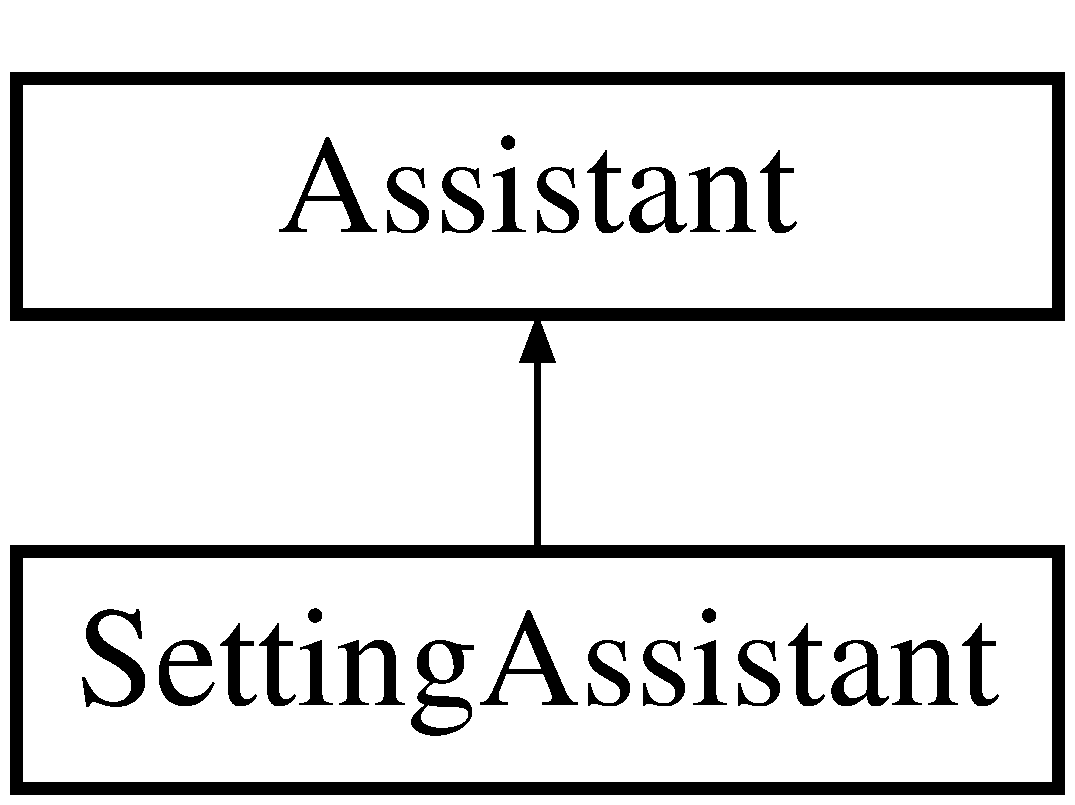
\includegraphics[height=2.000000cm]{classSettingAssistant}
\end{center}
\end{figure}
\subsection*{Public Member Functions}
\begin{DoxyCompactItemize}
\item 
\hypertarget{classSettingAssistant_a49c046dc76e8f275c482cab1c8cacb72}{{\bfseries Setting\-Assistant} (\hyperlink{structOptions}{Options} $\ast$opts, \hyperlink{classVideoGrabber}{Video\-Grabber} $\ast$video\-Grab, bool $\ast$was\-Aborted)}\label{classSettingAssistant_a49c046dc76e8f275c482cab1c8cacb72}

\end{DoxyCompactItemize}
\subsection*{Protected Member Functions}
\begin{DoxyCompactItemize}
\item 
\hypertarget{classSettingAssistant_a569252ccd0466898f7f58b4d801cbf98}{bool {\bfseries on\-\_\-delete\-\_\-event} (Gdk\-Event\-Any $\ast$event)}\label{classSettingAssistant_a569252ccd0466898f7f58b4d801cbf98}

\item 
\hypertarget{classSettingAssistant_ab72a75382318af97c2bc40e54398ad54}{void {\bfseries on\-\_\-quit} ()}\label{classSettingAssistant_ab72a75382318af97c2bc40e54398ad54}

\end{DoxyCompactItemize}


The documentation for this class was generated from the following files\-:\begin{DoxyCompactItemize}
\item 
headers/Setting\-Assistant.\-hpp\item 
src/Setting\-Assistant.\-cpp\end{DoxyCompactItemize}

\hypertarget{classTracker}{\section{Tracker Class Reference}
\label{classTracker}\index{Tracker@{Tracker}}
}
\subsection*{Public Member Functions}
\begin{DoxyCompactItemize}
\item 
\hypertarget{classTracker_afd3365f1a661b0d96ed091b1250ade34}{{\bfseries Tracker} (\hyperlink{classArea}{Area}, const std\-::string label, \hyperlink{structOptions}{Options} \&options)}\label{classTracker_afd3365f1a661b0d96ed091b1250ade34}

\item 
\hypertarget{classTracker_af8b257a9a2d5869d9a3c10448170dfe0}{void {\bfseries next\-Frame} (cv\-::\-Mat whole\-Frame, double time)}\label{classTracker_af8b257a9a2d5869d9a3c10448170dfe0}

\item 
\hypertarget{classTracker_a12bd9002e4999442279594633277692c}{bool {\bfseries get\-Is\-Valid} ()}\label{classTracker_a12bd9002e4999442279594633277692c}

\item 
\hypertarget{classTracker_a16d848b52d9d22537e383491d7bd57ae}{float {\bfseries get\-X} ()}\label{classTracker_a16d848b52d9d22537e383491d7bd57ae}

\item 
\hypertarget{classTracker_ac3c91b671be24b2ddca67dc95d08200a}{float {\bfseries get\-Y} ()}\label{classTracker_ac3c91b671be24b2ddca67dc95d08200a}

\item 
\hypertarget{classTracker_a48ac1ec6775187764fea452a78a91b18}{float {\bfseries get\-Likelyhood} ()}\label{classTracker_a48ac1ec6775187764fea452a78a91b18}

\item 
\hypertarget{classTracker_aa85827fe11d16eb2f5e28534b04d8270}{float {\bfseries get\-Trained\-Frac} ()}\label{classTracker_aa85827fe11d16eb2f5e28534b04d8270}

\item 
\hypertarget{classTracker_af1e6e9c0c7f279d90739faa8f6866525}{std\-::string {\bfseries get\-Label} ()}\label{classTracker_af1e6e9c0c7f279d90739faa8f6866525}

\item 
\hypertarget{classTracker_a9f4bea276b87d8659d948fa78e1e08d4}{int {\bfseries get\-Territ} ()}\label{classTracker_a9f4bea276b87d8659d948fa78e1e08d4}

\item 
\hypertarget{classTracker_aa27e4f7e9825f2c4940b12f455fdb093}{bool {\bfseries get\-Is\-Trained} ()}\label{classTracker_aa27e4f7e9825f2c4940b12f455fdb093}

\item 
\hypertarget{classTracker_a4967034e7a3513a4af95b028b1be0156}{cv\-::\-Mat \& {\bfseries get\-Territ\-Map} ()}\label{classTracker_a4967034e7a3513a4af95b028b1be0156}

\item 
\hypertarget{classTracker_a531a88b730fbde3d3133f57277754c72}{cv\-::\-Rect \& {\bfseries get\-R\-O\-I} ()}\label{classTracker_a531a88b730fbde3d3133f57277754c72}

\end{DoxyCompactItemize}


The documentation for this class was generated from the following files\-:\begin{DoxyCompactItemize}
\item 
headers/Tracker.\-hpp\item 
src/Tracker.\-cpp\end{DoxyCompactItemize}

\hypertarget{classVideoGrabber}{\section{Video\-Grabber Class Reference}
\label{classVideoGrabber}\index{Video\-Grabber@{Video\-Grabber}}
}
\subsection*{Public Member Functions}
\begin{DoxyCompactItemize}
\item 
\hypertarget{classVideoGrabber_a03ab200fc52862e086f9f2f22173a6f9}{{\bfseries Video\-Grabber} (\hyperlink{structOptions}{Options} $\ast$opts)}\label{classVideoGrabber_a03ab200fc52862e086f9f2f22173a6f9}

\item 
\hypertarget{classVideoGrabber_a3f6df7add151ffb2b073e71527940187}{bool {\bfseries reinit} (\hyperlink{structOptions}{Options} $\ast$opts)}\label{classVideoGrabber_a3f6df7add151ffb2b073e71527940187}

\item 
\hypertarget{classVideoGrabber_a81cc2257449d8c66cd064c140dcd9295}{bool {\bfseries get\-Frame} (cv\-::\-Mat \&img, double $\ast$time)}\label{classVideoGrabber_a81cc2257449d8c66cd064c140dcd9295}

\item 
\hypertarget{classVideoGrabber_a8b32688d649574146f297e6550a502af}{void {\bfseries reset} ()}\label{classVideoGrabber_a8b32688d649574146f297e6550a502af}

\item 
\hypertarget{classVideoGrabber_a45cda38c6cfae4e29fecb069df1da9c0}{int {\bfseries get\-F\-P\-S} ()}\label{classVideoGrabber_a45cda38c6cfae4e29fecb069df1da9c0}

\item 
\hypertarget{classVideoGrabber_a02fa68136ee360e22f82cff82f42d5a4}{double {\bfseries get\-Progress} ()}\label{classVideoGrabber_a02fa68136ee360e22f82cff82f42d5a4}

\end{DoxyCompactItemize}
\subsection*{Protected Member Functions}
\begin{DoxyCompactItemize}
\item 
\hypertarget{classVideoGrabber_aa12db82dbfc5d0d620bbb3082c3d658d}{long {\bfseries get\-Time\-Dev} ()}\label{classVideoGrabber_aa12db82dbfc5d0d620bbb3082c3d658d}

\end{DoxyCompactItemize}


The documentation for this class was generated from the following files\-:\begin{DoxyCompactItemize}
\item 
headers/Video\-Grabber.\-hpp\item 
src/Video\-Grabber.\-cpp\end{DoxyCompactItemize}

\hypertarget{classVideoWriter}{\section{Video\-Writer Class Reference}
\label{classVideoWriter}\index{Video\-Writer@{Video\-Writer}}
}
\subsection*{Public Member Functions}
\begin{DoxyCompactItemize}
\item 
\hypertarget{classVideoWriter_a1fa9229cdd19b8335935792388405be4}{{\bfseries Video\-Writer} (std\-::vector$<$ \hyperlink{classTracker}{Tracker} $>$ $\ast$trackers, \hyperlink{structOptions}{Options} \&options, cv\-::\-Size global\-Frame\-Size, int fps)}\label{classVideoWriter_a1fa9229cdd19b8335935792388405be4}

\item 
\hypertarget{classVideoWriter_a831b1acdd93024d4a5ef70c3bec2af14}{void {\bfseries new\-Frame} (cv\-::\-Mat \&frame)}\label{classVideoWriter_a831b1acdd93024d4a5ef70c3bec2af14}

\end{DoxyCompactItemize}


The documentation for this class was generated from the following files\-:\begin{DoxyCompactItemize}
\item 
headers/Video\-Writer.\-hpp\item 
src/Video\-Writer.\-cpp\end{DoxyCompactItemize}

\addcontentsline{toc}{part}{Index}
\printindex
\end{document}
